\documentclass[11pt, aspectratio=169, xcolor=table]{beamer}
\usepackage[utf8]{inputenc}
\usepackage[T1]{fontenc}
\usepackage{graphicx}
\usepackage{hyperref}
\usepackage{lmodern}
\usepackage[spanish]{babel}
\usepackage{pdfrender}
\usepackage{xcolor}
\usepackage{ragged2e}
\usepackage[version=4]{mhchem}
\usepackage{siunitx}
\usepackage{multirow}
\renewcommand{\raggedright}{\justifying}
\usepackage{smartdiagram}
\usetheme{Berlin}

\author{Prof. Daniel Muñoz \\
	\texttt{daniel.munoz3@mail.udp}
}
\title{Química Unidad 3}
\subtitle{¿Qué transformaciones químicas producen energía en la vida cotidiana?: Cambio y energía en la Química}

\begin{document}

\maketitle

\section{Termoquímica: Concepto de Entalpía}

\begin{frame}{Introducción}
	\begin{columns}
		\begin{column}{.5\textwidth}
			\begin{itemize}[<+->]
				\item La termoquímica es la rama de la química que estudia los cambios de energía, especialmente en forma de calor, que acompañan a los cambios en la materia.
				\item Este desarrollo está imbuido de un fuerte sistema matemático interpretativo el cual, revisaremos de forma extremadamente superficial.
			\end{itemize}
		\end{column}

		\begin{column}{.5\textwidth}
			\begin{figure}[ht]
				\centering
				\includegraphics[width=0.6\textwidth]{../img/termodinamics.png}
				\caption{\label{fig:label} Cuatro potenciales comunes: $H = U + PV$}
			\end{figure}

		\end{column}
	\end{columns}
\end{frame}

\begin{frame}{Historia: Los inicios de una rama}
	\begin{columns}
		\begin{column}{.5\textwidth}
			\begin{itemize}[<+->]
				\item Ingeniero francés, considerado el padre de la termodinámica.
				\item En 1824 publicó ``Reflexiones sobre la potencia motriz del fuego''.
				\item Introdujo el concepto, conocido actualmente como \texttt{ciclo de Carnot}, mostrando que la eficiencia máxima de una máquina térmica depende únicamente de las temperaturas entre las que opera, no del tipo de fluido o mecanismo.
			\end{itemize}
		\end{column}

		\begin{column}{.5\textwidth}
			\begin{figure}[ht]
				\centering
				\includegraphics[width=0.4\textwidth]{../img/carnot.png}
				\caption{\label{fig:label} Sadi Carnot (1796 - 1832) }
			\end{figure}

		\end{column}
	\end{columns}

\end{frame}

\begin{frame}{Historia: Inició el desorden.}

	\begin{columns}
		\begin{column}{.5\textwidth}
			\begin{itemize}[<+->]
				\item Físico alemán.
				\item Introdujo el concepto de energía interna ($U$) como propiedad del sistema.
				\item Enunció formalmente el \texttt{Segundo Principio de la Termodinámica} y definió la entropía ($S$).
				\item Descubrió que esta $U$ dependía de la temperatura, la presión y el volumen.
			\end{itemize}

		\end{column}

		\begin{column}{.5\textwidth}
			\begin{figure}[ht]
				\centering
				\includegraphics[width=0.6\textwidth]{../img/clasius.png}
				\caption{\label{fig:label} Rudolf Clasius (1822 - 1888)}
			\end{figure}

		\end{column}
	\end{columns}

\end{frame}

\begin{frame}{Historia: El signo de los tiempos}
	\begin{columns}
		\begin{column}{.5\textwidth}
			\begin{itemize}[<+->]
				\item Científico inglés que profundizó los alcances de la \textit{termodinámica}
				\item Creo la escala de temperatura absoluta (cuyas unidades llevan su nombre)
				\item Logró esclarecer la relación entre \textbf{trabajo}, \textbf{calor} y \textbf{energía}.
				\item ``La ciencia ya lo ha descubierto todo.''
			\end{itemize}
		\end{column}

		\begin{column}{.5\textwidth}
			\begin{figure}[ht]
				\centering
				\includegraphics[width=0.5\textwidth]{../img/kelvin.png}
				\caption{\label{fig:label} William Thomson (Lord Kelvin) (1824–1907)}
			\end{figure}

		\end{column}
	\end{columns}

\end{frame}

\begin{frame}[allowdisplaybreaks]
	\frametitle{Historia: Definición moderna de Entalpía}
	\begin{columns}
		\begin{column}{.5\textwidth}
			\begin{itemize}[<+->]
				\item Físico neerlandés, galardonado con el nobel de física en 1913.
				\item Descubrió la superconductividad y logró licuar helio.
				\item Fue el primero en usar el término ``entalpía'', $H$ (del griego ``agregar calor'').
				\item Formalizó el concepto con la fórmula $H = U + PV$.
			\end{itemize}
		\end{column}

		\begin{column}{.5\textwidth}
			\begin{figure}[ht]
				\centering
				\includegraphics[width=0.5\textwidth]{../img/onnes.png}
				\caption{\label{fig:label} Heike Kamerlingh Onnes (1853–1926)}
			\end{figure}

		\end{column}
	\end{columns}

\end{frame}

\begin{frame}[allowdisplaybreaks]
	\frametitle{Concepto de entalpía}
	\begin{columns}
		\begin{column}{.5\textwidth}
			\begin{itemize}[<+->]
				\item La entalpía de un sistema se define cómo: $H = U + PV$
				\item Dónde $U$ es:
				      \begin{itemize}[<+->]
					      \item La energía cinética microscópica (vibraciones, rotaciones, traslaciones, etc.)
					      \item La energía potencial microscópica (ff intermoleculares, enlaces, etc.)
				      \end{itemize}
				\item P es la presión del sistema (generalmente cte.)
				\item V es el volumen del sistema.
			\end{itemize}
		\end{column}

		\begin{column}{.5\textwidth}
			\only<7->{Pero como generalmente solamente se puede ver el cambio, entonces se prefiere la siguiente fórmula:\\}
			\only<8->{
			$H_{final}-H_{inicial}=\Delta H = \Delta U + P \Delta V$
			}
		\end{column}
	\end{columns}
\end{frame}

\begin{frame}[allowdisplaybreaks]
	\frametitle{Ejemplo}
	\begin{columns}
		\begin{column}{.5\textwidth}
			Un gas se expande a presión constante de \qty{2,0}{\litre} a \qty{3,0}{\litre}, la expansión de dio a una presión atmosférica constante de \qty{1,0}{atm}. Durante el proceso la energía interna del gas aumentó en \qty{400}{J}. Recuerde que \qty{1}{L.atm} = \qty{101,325}{J}
			\begin{exampleblock}<2->{Respuesta}
				\begin{itemize}[<+->]
					\small
					\item $\Delta U = \qty{400}{J}$
					\item $P = \qty{1}{atm} $
					\item $\Delta V = \qty{3,0}{L}-\qty{2,0}{L} = \qty{1,0}{L}$
					\item Reemplazamos en: $\Delta H = \Delta U + P \Delta V$
				\end{itemize}
			\end{exampleblock}
		\end{column}

		\begin{column}{.5\textwidth}
			\begin{exampleblock}<2->{}
				\begin{itemize}[<+->]
					\item Primero calcularemos $P \Delta V$ en J.
					\item $P \Delta V = (\qty{1,0}{atm})(\qty{1,0}{L}) = \qty{1,0}{L.atm}$
					\item $\qty{1,0}{L.atm} = \qty{101,325}{J}$
					\item Calculamos $\Delta H$:
					\item $\Delta H = \qty{400}{J} + \qty{101,725}{J}$
					\item $\Delta H = \qty{101,725}{J}$
					\item Como vemos el valor es positivo esto significa que el sistema perdió energía (se enfrió en el proceso)
				\end{itemize}
			\end{exampleblock}
		\end{column}
	\end{columns}
\end{frame}

\begin{frame}[allowdisplaybreaks]
	\frametitle{Expansión de un gas.}
	\begin{columns}
		\begin{column}{.5\textwidth}
			\begin{figure}[ht]
				\centering
				\includegraphics[width=0.6\textwidth]{../img/expansion-1.png}
				\caption{\label{fig:label} Expansión de un gas foto 1}
			\end{figure}
		\end{column}
		\begin{column}{.5\textwidth}
			\begin{figure}[ht]
				\centering
				\includegraphics[width=0.6\textwidth]{../img/expansion-2.png}
				\caption{\label{fig:label} Expansión de un gas foto 2}
			\end{figure}

		\end{column}
	\end{columns}

\end{frame}

\section{Clasificación de una reacción como endotérmica o exotérmica a partir del valor de entalpía.}

\begin{frame}[allowdisplaybreaks]
	\frametitle{Introducción a la Termodinámica Química}
	¡Hola a todos! En esta clase, exploraremos los fundamentos de la termodinámica química, centrándonos en la entalpía ($\Delta H$) y la entropía ($\Delta S$). Estos conceptos son esenciales para comprender los cambios de energía en las reacciones químicas y predecir su espontaneidad.

\end{frame}

\begin{frame}[allowdisplaybreaks]
	\frametitle{Entalpía $\Delta H$: El calor de Reacción}
	\begin{columns}
		\begin{column}{.5\textwidth}
			\scriptsize
			La entalpía (H) es una medida del contenido de calor de un sistema a presión constante. El cambio de entalpía ($\Delta H$) es el calor absorbido o liberado durante una reacción química:

			\begin{itemize}
				\scriptsize
				\item Reacción Exotérmica: $\Delta H < 0$. La reacción libera calor al entorno.
				\item Ejemplo: Combustión de un combustible.
				\item Reacción Endotérmica: $\Delta H > 0$. La reacción absorbe calor del entorno.
				\item Ejemplo: Fusión de hielo.
			\end{itemize}

			\textbf{Importancia}: $\Delta H$ nos permite cuantificar el calor involucrado en las reacciones, lo cual es crucial para el diseño de reactores químicos y la comprensión de procesos industriales.
		\end{column}

		\begin{column}{.5\textwidth}
			\begin{figure}[ht]
				\centering
				\includegraphics[width=\textwidth]{../img/exo-endo.png}
				\caption{\label{fig:label} Proceso exotérmico y endotérmico}
			\end{figure}

		\end{column}
	\end{columns}
\end{frame}

\begin{frame}[allowdisplaybreaks]
	\frametitle{Germain Henri Hess 1802 - 1850}
	\begin{columns}
		\begin{column}{.5\textwidth}
			\begin{itemize}[<+->]
				\item Químico y médico suizo formuló uno de los primeros principios en termoquímica
				\item Nació en Ginebra, pero se mudó a Rusia con su familia.
				\item Estudió en la universidad de Tartu graduándose como médico en 1825.
				\item Se interesó en la química después de conocer y trabajar con \textit{Berzelius}.
				\item 1830 presenta su trabajo ``Ley de suma constante del calor'' (hoy conocida como Ley de Hess).
			\end{itemize}
		\end{column}

		\begin{column}{.5\textwidth}
			\begin{figure}[ht]
				\centering
				\includegraphics[height=.6\textheight]{../img/hess.png}
				\caption{\label{fig:label} 1802 - 1850 (48 años)}
			\end{figure}

		\end{column}
	\end{columns}

\end{frame}

\section{Cálculo de valores termodinámicos empleando la ley de Hess.}

\begin{frame}[allowdisplaybreaks]
	\frametitle{Cálculo de $\Delta H$: Ley de Hess}
	\begin{columns}
		\begin{column}{.5\textwidth}
			\scriptsize
			La Ley de Hess establece que el cambio de entalpía para una reacción es independiente del número de pasos en que se produce la reacción. Esto nos permite calcular $\Delta H$ para reacciones que no se pueden medir directamente.
			\begin{alertblock}{}
				Los elementos ej: \ce{Cl2}, \ce{O2}, \ce{Na}, etc. tiene $\Delta H_{f} = 0$
			\end{alertblock}

			\begin{exampleblock}{Ejemplo}
				\scriptsize
				Calcular la entalpía de formación del etano \ce{C2H6} y determine si libera o absorbe calor:
				\begin{enumerate}
					\item \ce{C2H6(g) + 7/2O2(g) -> 2CO2(g) + 3H2O(l)} $\Delta H_{1}=\qty{-1560}{kJ}$
					\item \ce{C(s) + O2(g) -> CO2(g)} $\Delta H_{2} = \qty{-393,5}{kJ}$
					\item \ce{H2(g) + 1/2O2(g) -> H2O(l)} $\Delta H_{3} = \qty{-286,0}{kJ}$
				\end{enumerate}
			\end{exampleblock}

		\end{column}

		\begin{column}{.5\textwidth}

		\end{column}
	\end{columns}

\end{frame}

\begin{frame}[allowdisplaybreaks]
	\frametitle{Aplicaciones de la Entalpía}
	\begin{columns}
		\begin{column}{.5\textwidth}
			\begin{itemize}
				\scriptsize
				\item 1890: La industria del salitre desde finales del siglo XIX y principios del XX generaron enormes ingresos para Chile, los cuales correspondieron hasta un 70\% de los ingresos fiscales.
				\item 1910: Carl Bosh desarrolla el proceso de \textit{Haber-Bosh}
				\item 1914-1918: Estalla la primera guerra mundial, y Alemania sufre el bloqueo de compra de salitre por Inglaterra, en ese período Alemania prescinde el salitre, principalmente Chileno, al desarrollar el propio de forma sintética.
				\item 1929: La gran crisis económica y las bajas rentabilidades de la extracción del salitre provocan el fin de la industria salitrera en Chile.
			\end{itemize}
		\end{column}

		\begin{column}{.5\textwidth}
			\begin{figure}[ht]
				\centering
				\includegraphics[width=0.8\textwidth]{../img/haber-bosh.png}
				\caption{\label{fig:label} Proceso de síntesis de amoniaco}
			\end{figure}

		\end{column}
	\end{columns}
\end{frame}

\section{Entropía y Energía libre de Gibbs}

\begin{frame}[allowdisplaybreaks]
	\frametitle{Entropía $\Delta S$: El desorden molecular}

	\begin{columns}
		\begin{column}{.5\textwidth}
			\scriptsize
			La entropía (S) es una medida del desorden o aleatoriedad de un sistema. El cambio de entropía ($\Delta S$) nos indica si el desorden del sistema aumenta o disminuye durante un proceso.

			\begin{itemize}
				\scriptsize
				\item $\Delta S > 0$: Aumento del desorden.
				\item Ejemplos: Fusión, evaporación, aumento del número de moles de gas.
				\item $\Delta S < 0$: Disminución del desorden.
				\item Ejemplos: Condensación, congelación.
			\end{itemize}

			\textbf{¿Quién definió la entropía?} Si bien varios científicos contribuyeron, \textit{Ludwig Boltzmann} hizo contribuciones significativas al conectar la entropía con la probabilidad y el número de microestados de un sistema.
			\\\textbf{Importancia:} La entropía es un factor clave que determina la espontaneidad de las reacciones.

		\end{column}

		\begin{column}{.5\textwidth}
			\begin{figure}[ht]
				\centering
				\includegraphics[width=.8\textwidth]{../img/entropia.png}
				\caption{\label{fig:label} Cambio de entropía/desorden}
			\end{figure}

		\end{column}
	\end{columns}
\end{frame}

\begin{frame}[allowdisplaybreaks]
	\frametitle{Ludwing Boltzman: 1844 - 1906}
	\begin{columns}
		\begin{column}{.5\textwidth}
			\begin{itemize}
				\scriptsize
				\item Físico Austriaco padre de la mecánica estadística.
				\item Desarrollo el concepto actualmente usado de entropía.
				\item Logró vincular propiedades macroscópicas con microscópicas mediante tratamientos estadísticos.
				\item Sus trabajos fueron continuados posteriormente por Einstein y defendidos por Planck.
				\item En 1906 se suicida, según mencionan, por falta de reconocimiento.
			\end{itemize}
		\end{column}

		\begin{column}{.5\textwidth}
			\begin{figure}[ht]
				\centering
				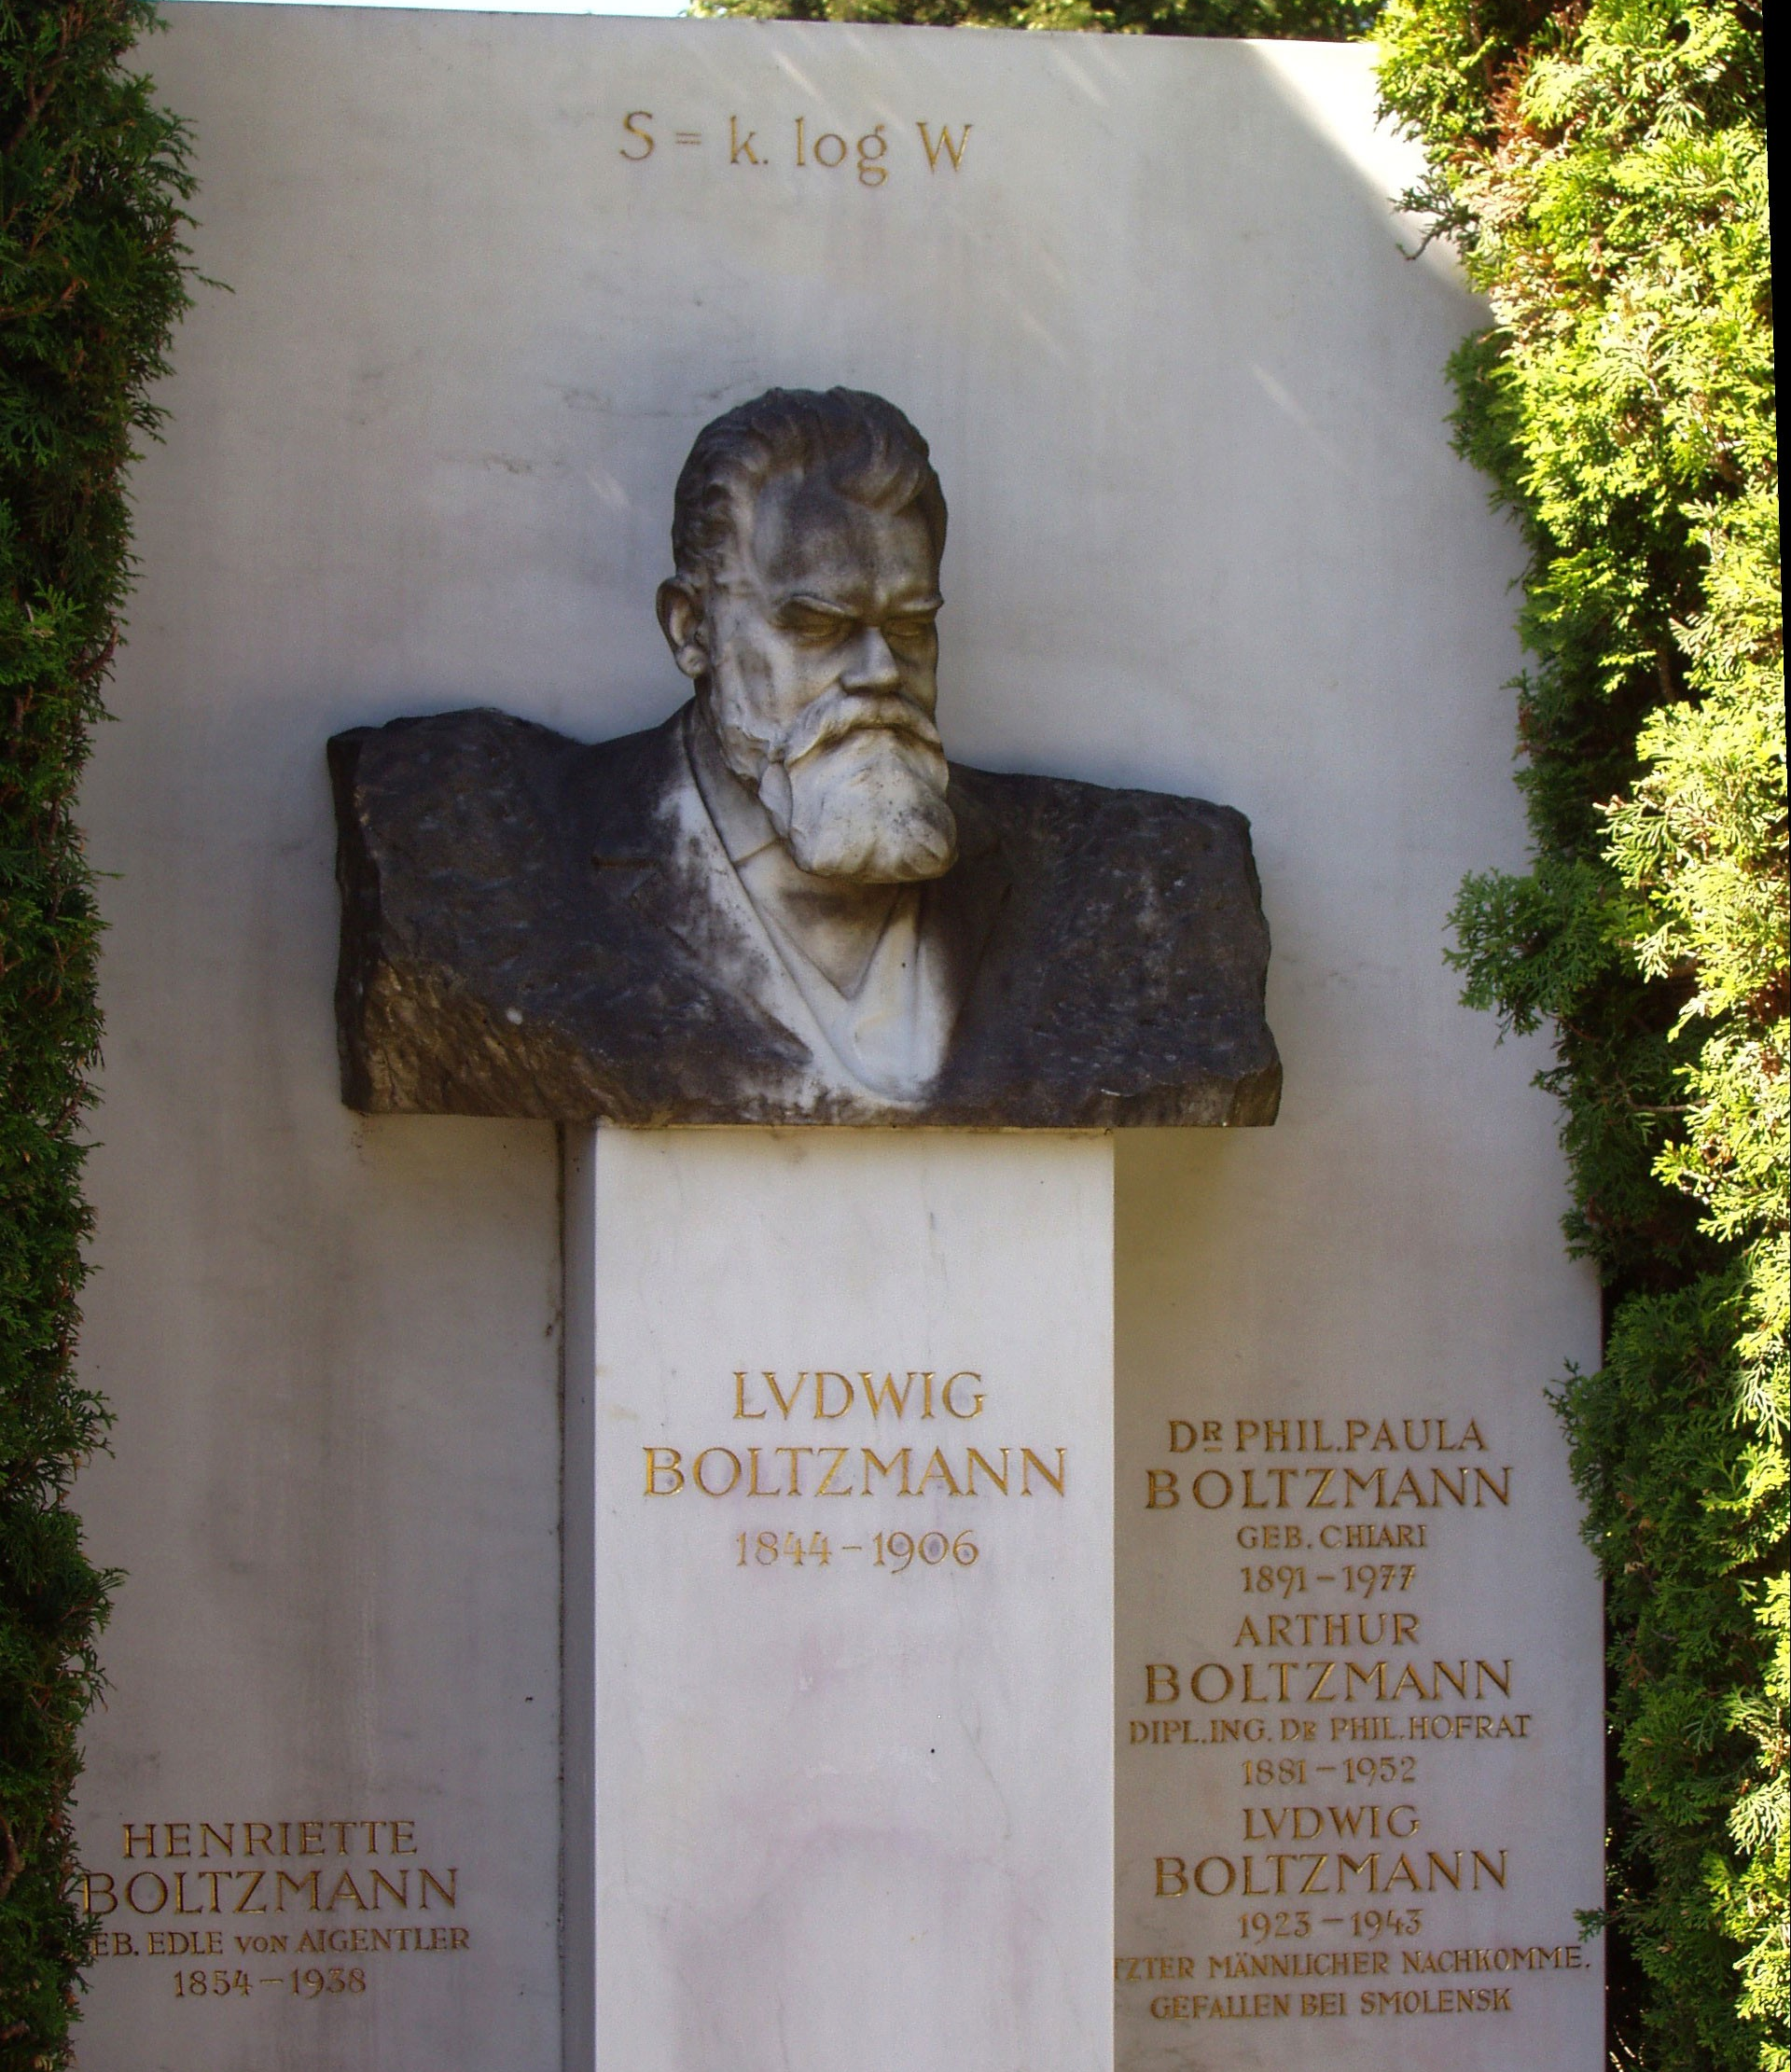
\includegraphics[height=0.6\textheight]{../img/boltzman.png}
				\caption{\label{fig:label} Tumba de Boltzman en Viena}
			\end{figure}

		\end{column}
	\end{columns}
\end{frame}

\begin{frame}[allowdisplaybreaks]
	\frametitle{Predicción del cambio de entropía $\Delta S$}

	\begin{columns}
		\begin{column}{.5\textwidth}
			La entropía aumenta ($\Delta S$) cuando en un cambio:
			\begin{itemize}
				\item El cambio de fase es: \ce{S -> L -> G}.
				\item Aumenta del número de moles gas.
			\end{itemize}
			Por tanto disminuirá ($\Delta S < 0$) cuando es lo opuesto.
		\end{column}
		\begin{column}{.5\textwidth}
			\begin{exampleblock}{Ejemplo}
				Determine el cambio de entropía para los siguientes procesos:
				\begin{itemize}
					\item \ce{I2(s) -> I2(g)}
					\item \ce{4Fe(s) + 3O2(g) -> 2Fe2O3(s)}
				\end{itemize}
			\end{exampleblock}
		\end{column}
	\end{columns}

\end{frame}


\begin{frame}[allowdisplaybreaks]
	\frametitle{Cálculo de $\Delta S$}

	\begin{columns}
		\begin{column}{.5\textwidth}
			El cambio de entropía estándar de una reacción ($\Delta S_{reacción}$) se puede calcular a partir de las entropías estándar de los productos y los reactivos:
			\\$\Delta S_{reaccción}= \sum S^{0} (productos) - \sum S^{0} (reactivos)$
		\end{column}

		\begin{column}{.5\textwidth}
			\begin{exampleblock}{Ejemplo}
				Determine la entropía de la siguiente reacción:
				\\\centering \ce{N2(g) + 3H2(g) -> 2NH3(g)}

				Sabiendo que las entropías son:
				\begin{itemize}
					\item \ce{N2(g)}: \qty{191,50}{J/mol.K}
					\item \ce{H2(g)}: \qty{130,575}{J/mol.K}
					\item \ce{NH3(g)}:  \qty{192,34}{J/mol.K}
				\end{itemize}
			\end{exampleblock}

		\end{column}
	\end{columns}

\end{frame}

\section{Definición de la espontaneidad a partir de cálculos energía libre de Gibbs a partir de valores de entalpía y entropía a una temperatura dada}

\begin{frame}[allowdisplaybreaks]
	\frametitle{Energía Libre de Gibbs ($\Delta G$): Espontaneidad}

	\begin{columns}
		\begin{column}{.5\textwidth}
			La energía libre de Gibbs (G), desarrollada por \textit{Josiah Willard Gibbs}, combina entalpía (H) y entropía (S) para predecir la espontaneidad de una reacción:
			\\\centering $\Delta G = \Delta H - T\Delta S$
			\begin{itemize}
				\item $\Delta G <0$: Reacción espontánea
				\item $\Delta G > 0$: Reacción no espontánea
				\item $\Delta G = 0$: Reacción en equilibrio (esta ocurriendo en ambos sentidos a la vez.)
			\end{itemize}
		\end{column}

		\begin{column}{.5\textwidth}
			\begin{figure}[ht]
				\centering
				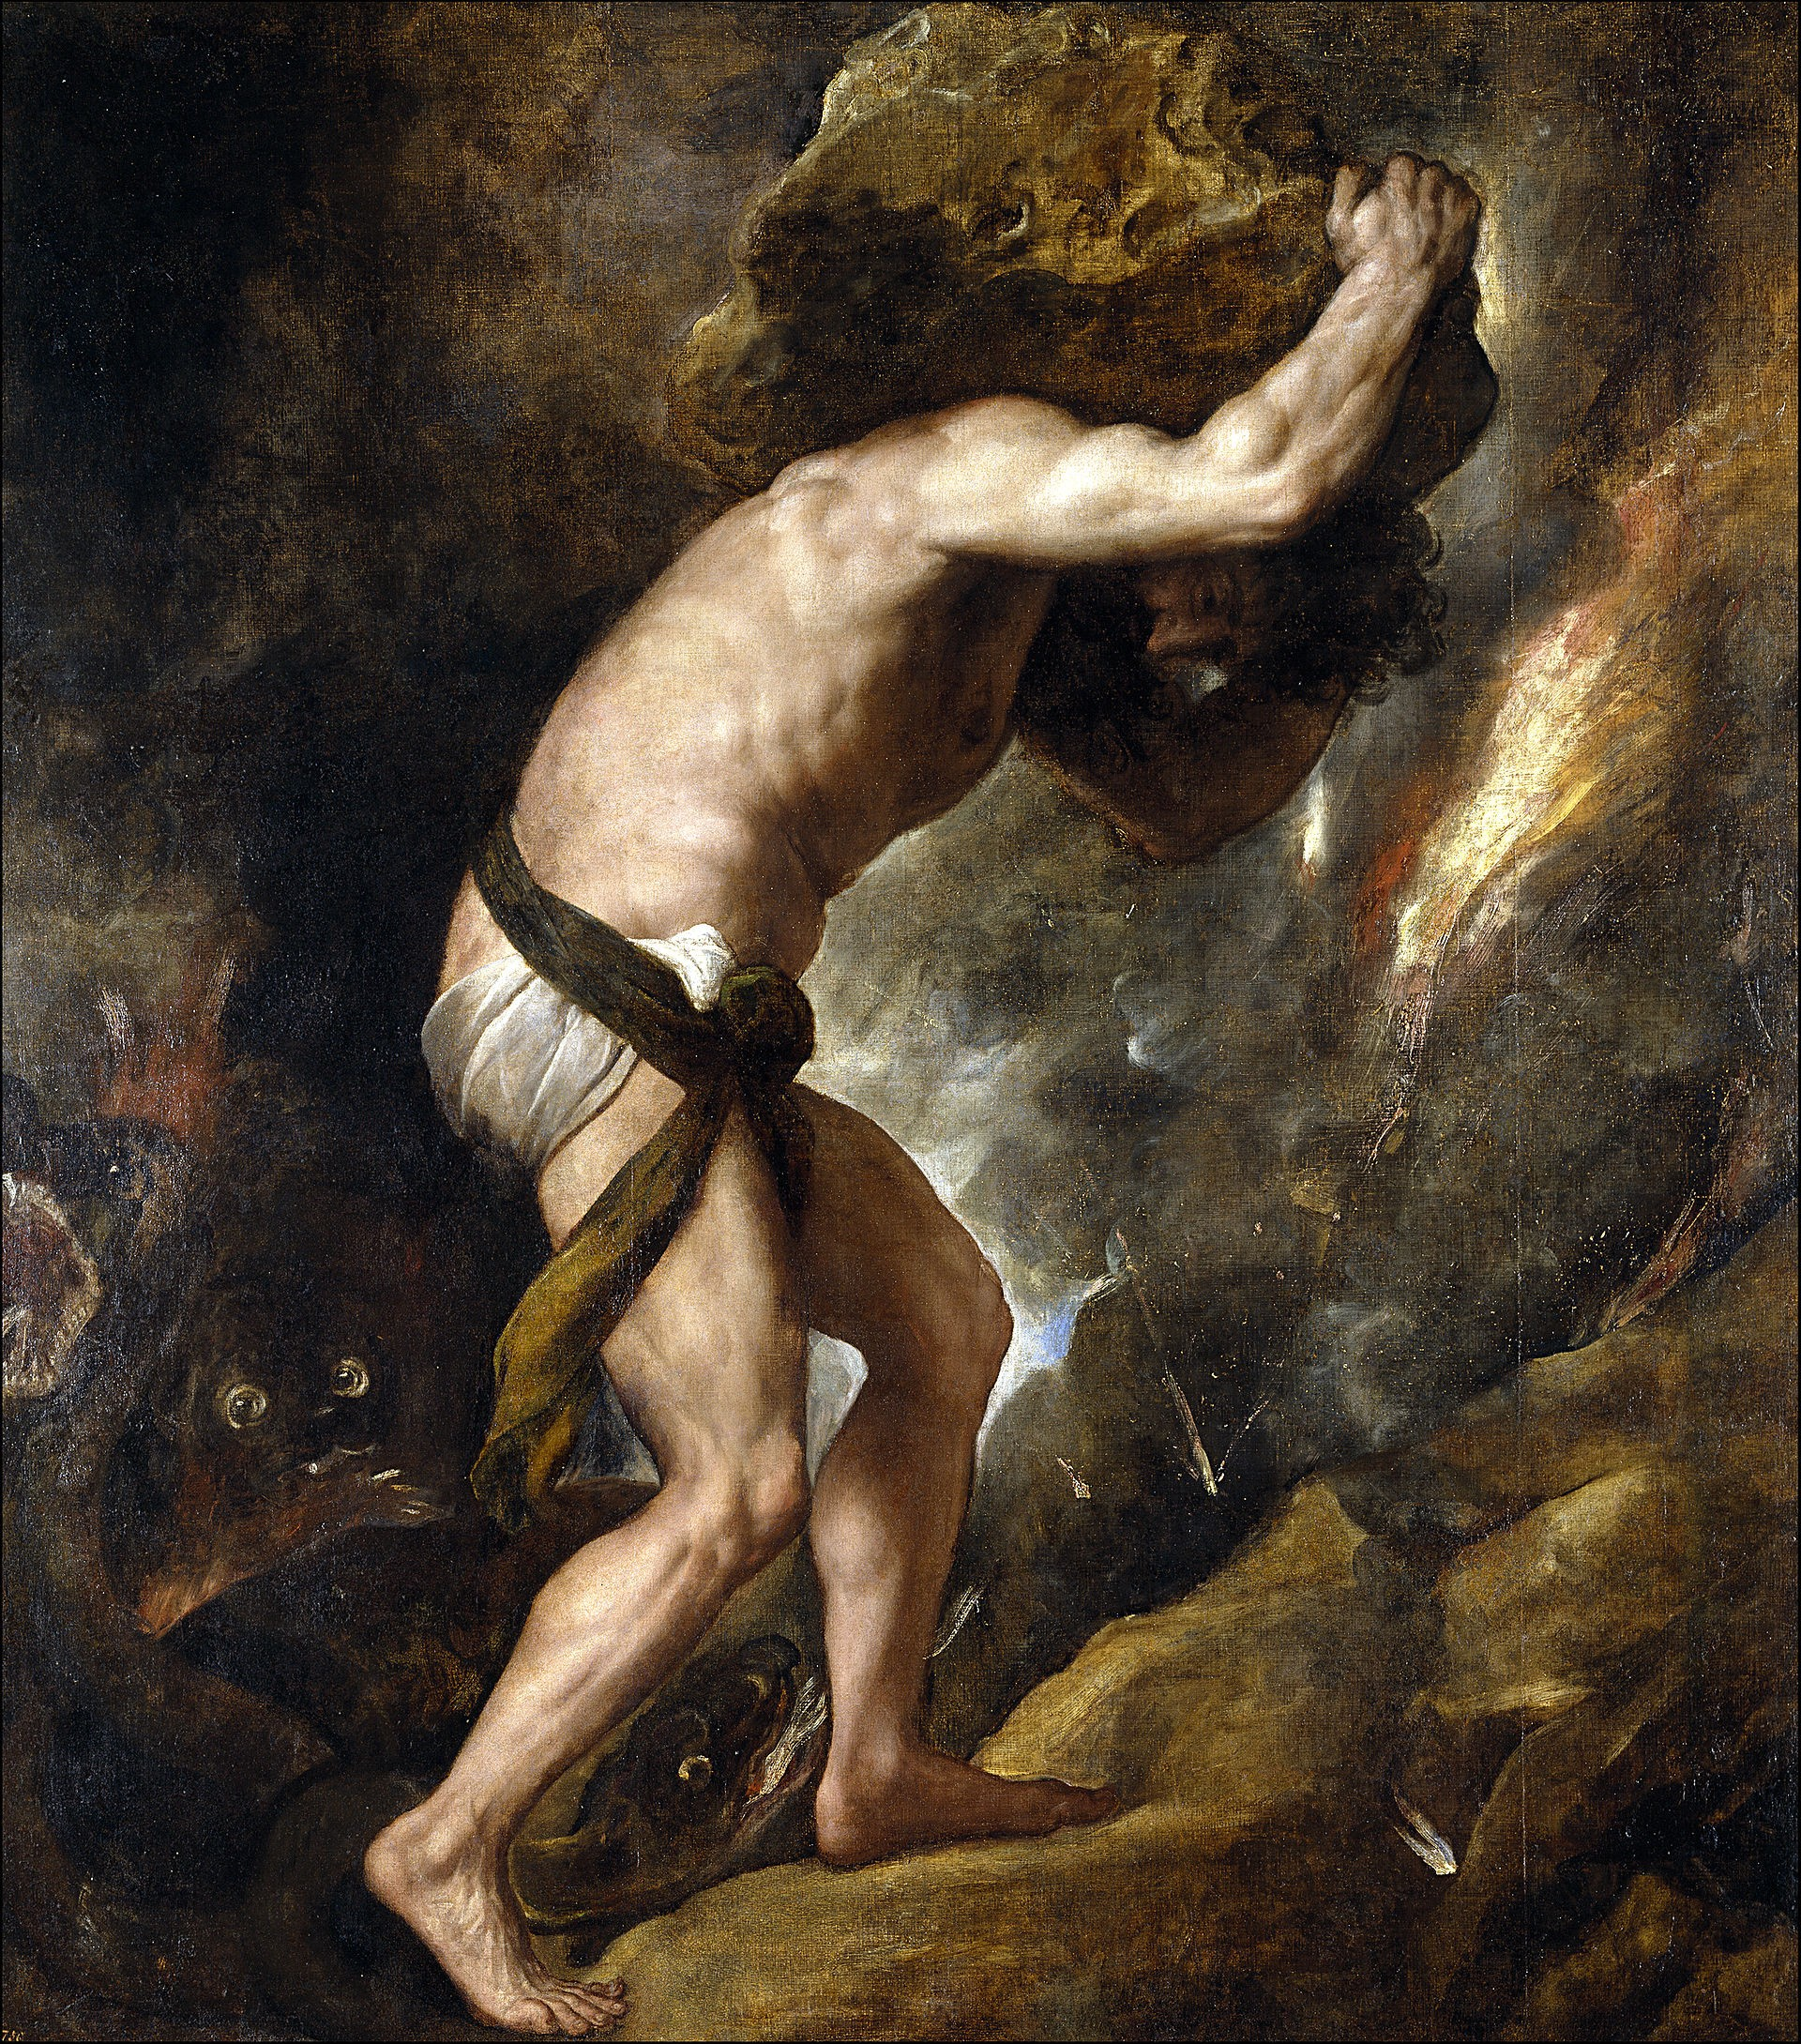
\includegraphics[width=.6\textwidth]{../img/no-espontaneo.png}
				\caption{\label{fig:label} Tiziano 1548. Sísifo}
			\end{figure}

		\end{column}
	\end{columns}
\end{frame}

\begin{frame}[allowdisplaybreaks]
	\frametitle{Josiah Williard Gibbs}
	\begin{columns}
		\begin{column}{.5\textwidth}
			\begin{itemize}
				\small
				\item físico estadounidense que contribuyó al desarrollo de la termodinámica.
				\item 1837 realizó una representación geométrica de las funciones de estado, trabajo bien recibido por el galardonado físico británico \textit{James Maxwell}.
				\item Hizo contribuciones en óptica, física matemática y crea la noción de potencial químico.
				\item En palabras de Einstein ``El mayor espíritu en la historia de América''
			\end{itemize}
		\end{column}

		\begin{column}{.5\textwidth}
			\begin{figure}[ht]
				\centering
				\includegraphics[width=.5\textwidth]{../img/gibbs.png}
				\caption{\label{fig:label} 1839 - 1903}
			\end{figure}

		\end{column}
	\end{columns}

\end{frame}

\begin{frame}[allowdisplaybreaks]
	\frametitle{Cálculo de $\Delta G$}
	\begin{columns}
		\begin{column}{.6\textwidth}
			\begin{exampleblock}{Ejemplo}
				Determine la energía libre de gibbs a \qty{25}{\degreeCelsius} para la reacción:
				\\\centering \ce{C2H4(g) + 3O2(g) -> 2H2O(g) + 2CO2(g)}
				\begin{table}[]
					\begin{tabular}{|l|l|l|}
						\hline
						          & H (\unit{kJ/mol}) & S (\unit{J/mol.K}) \\ \hline
						\ce{C2H4} & 52,3              & 209                \\ \hline
						\ce{O2}   & 0                 & 205,029            \\ \hline
						\ce{H2O}  & -241,818          & 188,716            \\ \hline
						\ce{CO2}  & -393,509          & 213,63             \\ \hline
					\end{tabular}
				\end{table}
			\end{exampleblock}

		\end{column}

		\begin{column}{.4\textwidth}

		\end{column}
	\end{columns}
\end{frame}

\begin{frame}[allowdisplaybreaks]
	\frametitle{Factores que afectan la espontaneidad}
	\begin{columns}
		\begin{column}{.5\textwidth}
			\begin{itemize}
				\item $\Delta H < 0$ y $\Delta S > 0$, la reacción es espontánea a todas las temperaturas
				\item $\Delta H > 0$ y $\Delta S < 0$, la reacción no es espontánea a ninguna temperatura.
				\item $\Delta H$ y $\Delta S$ tienen el mismo signo, la espontaneidad depende de la temperatura.
			\end{itemize}
		\end{column}

		\begin{column}{.5\textwidth}
			% Please add the following required packages to your document preamble:
			% \usepackage{multirow}
			\begin{table}[]
				\begin{tabular}{c|c|c|}
					\cline{2-3}
					                                                   & Desorden                          & Orden                       \\ \hline
					\multicolumn{1}{|l|}{\multirow{2}{*}{Exotérmica}}  & \multirow{2}{*}{$(-)$}         & $\uparrow T \Rightarrow (+)$   \\ \cline{3-3}
					\multicolumn{1}{|l|}{}                             &                                & $\downarrow T \Rightarrow (-)$ \\ \hline
					\multicolumn{1}{|l|}{\multirow{2}{*}{Endotérmica}} & $\uparrow T \Rightarrow (-)$   & \multirow{2}{*}{$(+)$}         \\ \cline{2-2}
					\multicolumn{1}{|l|}{}                             & $\downarrow T \Rightarrow (+)$ &                                \\ \hline
				\end{tabular}
			\end{table}
		\end{column}
	\end{columns}

\end{frame}

\begin{frame}[allowdisplaybreaks]
	\frametitle{Ejemplos de Espontaneidad y $\Delta G$}
	\begin{columns}
		\begin{column}{.6\textwidth}
			\begin{exampleblock}{Ejemplo}
				Determine a qué temperatura la siguiente reacción está en equilibrio, será espontánea y no espontánea:
				\\\centering \ce{2NaHCO3(s) -> Na2CO3(s) + CO2(g) + H2O(g)}
				\begin{table}[]
					\begin{tabular}{|l|l|l|}
						\hline
						               & $\Delta H$ (\unit{kJ/mol}) & $\Delta S$ (\unit{J/mol.K}) \\ \hline
						\ce{NaHCO3(s)} & -947,67                    & 102,09                      \\ \hline
						\ce{Na2CO3(s)} & -1130,9                    & 135,98                      \\ \hline
						\ce{CO2(g)}    & -393,50                    & 213,68                      \\ \hline
						\ce{H2O(g)}    & -241,82                    & 188,72                      \\ \hline
					\end{tabular}
				\end{table}
			\end{exampleblock}

		\end{column}

		\begin{column}{.4\textwidth}

		\end{column}
	\end{columns}
\end{frame}

\end{document}
